%%%%%%%%%%%%%%%%%%%%%%%%%%%%%%%%%%%%%%%%%
% Stylish Curriculum Vitae
% LaTeX Template
% Version 1.0 (18/7/12)
%
% This template has been downloaded from:
% http://www.LaTeXTemplates.com
%
% Original author:
% Stefano (http://stefano.italians.nl/)
%
% Modified by:
% Johan Angelstam (http://github.com/angelstam)
%
% IMPORTANT: THIS TEMPLATE NEEDS TO BE COMPILED WITH XeLaTeX
%
% License:
% CC BY-NC-SA 3.0 (http://creativecommons.org/licenses/by-nc-sa/3.0/)
%
% The main font used in this template, Adobe Garamond Pro, does not 
% come with Windows by default. You will need to download it in
% order to get an output as in the preview PDF. Otherwise, change this 
% font to one that does come with Windows or comment out the font line 
% to use the default LaTeX font.
%
%%%%%%%%%%%%%%%%%%%%%%%%%%%%%%%%%%%%%%%%%

\documentclass[a4paper, oneside, final]{scrartcl} % Paper options using the scrartcl class

\usepackage{scrpage2} % Provides headers and footers configuration
\usepackage{titlesec} % Allows creating custom \section's
\usepackage{marvosym} % Allows the use of symbols
\usepackage{tabularx,colortbl} % Advanced table configurations
\usepackage{fontspec} % Allows font customization

\usepackage{paralist} % Provides compact lists
\setdefaultleftmargin{1em}{1em}{1em}{1em}{1em}{1em}

\usepackage{tikz} % Rounded corners

\defaultfontfeatures{Mapping=tex-text}
\setmainfont{Adobe Garamond Pro} % Main document font

\titleformat{\section}{\large\scshape\raggedright}{}{0em}{}[\titlerule] % Section formatting

\pagestyle{scrheadings} % Print the headers and footers on all pages

\addtolength{\voffset}{-0.5in} % Adjust the vertical offset - less whitespace at the top of the page
\addtolength{\textheight}{3cm} % Adjust the text height - less whitespace at the bottom of the page

\newcommand{\gray}{\rowcolor[gray]{.90}} % Custom highlighting for the work experience and education sections

%---------------------------------------------------------------------
%  FOOTER SECTION
%---------------------------------------------------------------------

\renewcommand{\headfont}{\normalfont\rmfamily\scshape} % Font settings for footer

\cofoot{
\addfontfeature{LetterSpace=20.0}\fontsize{12.5}{17}\selectfont % Letter spacing and font size

Alsättersgatan 15 C.35 {\large\textperiodcentered} 584 35 Linköping {\large\textperiodcentered} Sweden\\ % Your mailing address
{\Large\Letter} johan@angelstam.se \ {\Large\Telefon} +46(0)70-308 24
94 \\ % Your email address and phone number

}

%---------------------------------------------------------------------

\begin{document}

\begin{center} % Center everything in the document

%---------------------------------------------------------------------
%  HEADER SECTION
%---------------------------------------------------------------------

{\addfontfeature{LetterSpace=20.0}\fontsize{36}{36}\selectfont\scshape
  Johan Angelstam} % Your name at the top

\vspace{1.2cm} % Extra whitespace after the large name at the top

%---------------------------------------------------------------------
%	OBJECTIVE
%---------------------------------------------------------------------

%\section{Objective}

%A position in the field of computers with special interests in
%business applications \\ programming, information processing, and
%management systems. 

%---------------------------------------------------------------------
%	WORK EXPERIENCE
%---------------------------------------------------------------------

\section{Work Experience}


\begin{tikzpicture}
\node (table) [inner sep=0mm] {
\begin{tabularx}{0.97\linewidth}{>{\raggedleft\scshape}p{2cm}X}
 Period & \textbf{August 2006 --- Present (Part Time)}\\
 Employer & \textbf{Followit Lindesberg AB} \hfill Lindesberg, Sweden\\
 Job Title & \textbf{Developer}\\
 Languages & \textbf{PHP, MySQL, Java (J2ME), C}\\
\end{tabularx}};
%\clip [rounded corners=.5cm] (0,0) rectangle coordinate (centerpoint) (5,7.5cm); 
\draw [gray, rounded corners=1mm, line width=0mm, fill=gray, opacity=.1] 
  (table.north west) rectangle (table.south east);
\end{tikzpicture}
\begin{tabularx}{0.97\linewidth}{X}
 I have gathered work experience in the following areas:
\begin{compactitem}
  \item Creating three generations of systems for receiving data from
    GPS-tracking units sending data by SMS, GPRS and the Iridium
    commercial communication satellite system format SBD.
    The systems, written in PHP, store the received data in a MySQL
    database, contain a web based administration, customer website
    with maps (Google, WMS and ArcIMS maps), the ability to forward
    data to the customers e-mail and production support
    systems. Responsable for continuously supporting, running,
    maintaining and improving the systems, on Linux and Windows
    servers.
  \item Creating a mobile client created with Java, connected to
    one of the above systems, used by hunters to track their dogs
    position.
  \item Creating several web sites using PHP and the Smarty templating
    system.
  \item Designing and creating product sheets with Adobe
    Illustrator/InDesign/Photoshop and films with Adobe Premiere/After
    Effects to demo GPS data visualized by Google Earth.
  \item Some experience coding for Microchip PIC18 in C.
\end{compactitem}
\end{tabularx}

%\vspace{12pt} % Empty line

\begin{tikzpicture}
\node (table) [inner sep=0mm] {
\begin{tabularx}{0.97\linewidth}{>{\raggedleft\scshape}p{2cm}X}
 Period & \textbf{May 2011 --- Present (Part Time)}\\
 Employer & \textbf{Linköping University} \hfill Linköping, Sweden\\
 Job Title & \textbf{Laboration Assistent}\\
\end{tabularx}};
%\clip [rounded corners=.5cm] (0,0) rectangle coordinate (centerpoint) (5,7.5cm); 
\draw [gray, rounded corners=1mm, line width=0mm, fill=gray, opacity=.1] 
  (table.north west) rectangle (table.south east);
\end{tikzpicture}
\begin{tabularx}{0.97\linewidth}{X}
Responsable for arranging study visits to different organizations and
companies as a part of a course at the Department of Electrical
Engineering.
\end{tabularx}

%---------------------------------------------------------------------
%	EDUCATION
%---------------------------------------------------------------------

\section{Education}

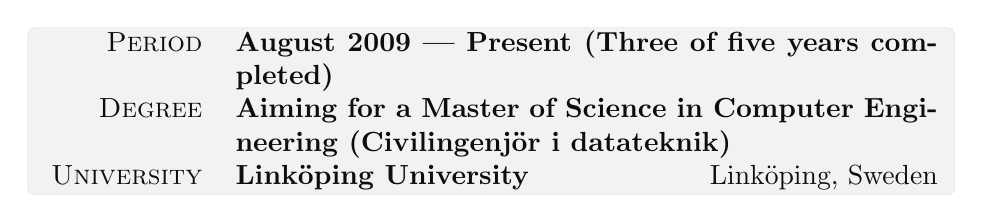
\begin{tikzpicture}
\node (table) [inner sep=0mm] {
\begin{tabularx}{0.97\linewidth}{>{\raggedleft\scshape}p{2cm}X}
 Period & \textbf{August 2009 --- Present (Three of
  five years completed)}\\
 Degree & \textbf{Aiming for a Master of Science in Computer
  Engineering (Civilingenjör i datateknik)}\\
 University & \textbf{Linköping University} \hfill Linköping, Sweden\\
%& Extra information about degree
\end{tabularx}};
%\clip [rounded corners=.5cm] (0,0) rectangle coordinate (centerpoint) (5,7.5cm); 
\draw [gray, rounded corners=1mm, line width=0mm, fill=gray, opacity=.1] 
  (table.north west) rectangle (table.south east);
\end{tikzpicture}

\vspace{10pt}


\begin{tikzpicture}
\node (table) [inner sep=0mm] {
\begin{tabularx}{0.97\linewidth}{>{\raggedleft\scshape}p{2cm}X}
 Period & \textbf{August 2001 --- December 2006}\\
 Degree & \textbf{Upper Secondary School - Natural Science}\\
 School & \textbf{Lindeskolan} \hfill Lindesberg, Sweden\\
%& Extra information about degree
\end{tabularx}};
%\clip [rounded corners=.5cm] (0,0) rectangle coordinate (centerpoint) (5,7.5cm); 
\draw [gray, rounded corners=1mm, line width=0mm, fill=gray, opacity=.1] 
  (table.north west) rectangle (table.south east);
\end{tikzpicture}

%---------------------------------------------------------------------
%	SKILLS
%---------------------------------------------------------------------

\section{Computer Skills}

\begin{tabular}{ @{} >{\bfseries}l @{\hspace{6ex}} l }
Computer Languages & PHP, Java, C, Objective-C, Lisp, VHDL, Ada \\
%Protocols \& APIs & XML, JSON, SOAP, REST \\
Databases & MySQL, Filemaker \\
Operating Systems & Unix (Linux, Solaris, NetBSD), Mac OS X\\
Tools & Git, Latex, Emacs, Eclipse, Xcode, Trac
\end{tabular}

%---------------------------------------------------------------------

\end{center}

\end{document}